
\chapter[Introdução]{Introdução}

Este capítulo tem como objetivo introduzir o leitor(a) aos temas principais que serão abordados neste trabalho. São apresentados conceitos como manutenibilidade de software, 
modelos de qualidade e \textit{code smells}, além de delimitar o escopo do problema, explicitar a 
pergunta de pesquisa que orienta a investigação e descrever a organização geral do documento.

\section{Contexto}

Avaliar a qualidade de produtos de \textit{software} é essencial para orientar decisões de projeto, reduzir 
subjetividades e padronizar a medição de atributos ao longo do ciclo de vida. Os primeiros referenciais surgiram 
com o modelo de \citeonline{McCall77}, que organizou fatores e subfatores de qualidade e propôs um método de 
avaliação quantitativa. Em seguida, \citeonline{boehm1978characteristics} ampliaram e sistematizaram essas ideias, 
estabelecendo uma base conceitual que influenciou normas posteriores. A \citeonline{ISOIEC9126} consolidou um 
vocabulário comum e, mais tarde, a \citeonline{ISOIEC25010} atualizou a taxonomia e introduziu a distinção entre 
qualidade interna, externa e em uso, destacando \textit{manutenibilidade} como característica de primeira ordem 
composta, entre outras, por \textit{analisabilidade}, \textit{modificabilidade} e \textit{testabilidade}.

Operacionalizar essas características exige métricas e instrumentos capazes de aproximar os modelos conceituais 
da realidade do código-fonte. Nesse ponto emergem os \textit{code smells}, originalmente descritos por \citeonline{Fowler1999}, 
como sinais recorrentes de problemas de projeto e implementação (por exemplo, \textit{Long Method}, \textit{God Class}, 
\textit{Feature Envy}, \textit{Data Class}). Embora não sejam defeitos funcionais, tais indícios estão associados a maior 
esforço de manutenção, risco de introdução de erros e degradação de atributos da qualidade interna \cite{Lanza2006}. 
Assim, mapear e tratar \textit{smells} torna-se um caminho prático para apoiar a \textit{analisabilidade} prevista nos modelos de qualidade.

Ferramentas de análise estática, como SonarQube, PMD, Checkstyle e SpotBugs, difundiram-se como meios de detectar \textit{smells} e 
antipadrões por meio de regras, métricas e limiares \cite{sonarq,pmdbox,checkstyle,spotbugs}. Elas oferecem velocidade, 
fácil integração a \textit{pipelines} de CI/CD e ampla cobertura de regras. Contudo, sua natureza heurística pode gerar 
taxas relevantes de falsos positivos, sensibilidade limitada ao contexto do sistema e dificuldade para capturar indícios 
mais sutis ou dependentes de semântica e histórico de evolução \cite{Sjoberg2013,Palomba2018}. Esses limites motivam a 
busca por abordagens mais adaptativas.

Nos últimos anos, com a popularização da Inteligência Artificial (IA), houve um aumento na aplicação de técnicas de IA na detecção e análise 
de \textit{code smells}. Abordagens 
incluem aprendizado supervisionado com métricas de código e AST, modelos baseados em 
representações estruturais (grafos, \textit{code embeddings}), \textit{deep learning} e, mais recentemente, 
\textit{Large Language Models} (LLMs).

Ao articular modelos de qualidade clássicos (McCall, Boehm, ISO) com a prática contemporânea de detecção de \textit{code smells}, 
este estudo busca fornecer uma síntese crítica e baseada em evidências sobre a real contribuição das técnicas de IA em especial 
LLMs frente às ferramentas estáticas tradicionais, indicando oportunidades concretas de pesquisa e de adoção em ambientes de desenvolvimento.

\section{Problema}

A seguir são apresentadas as orientações básicas sobre a formatação do
documento. O modelo \LaTeX\ \textbf{já configura todas estas opções corretamente},
de modo que para os usuários deste modelo o texto de toda esta Seção é 
\textbf{meramente informativo}.

\section{Questão de Pesquisa}

\label{qp_principal}

A pergunta de pesquisa foi construída com base na metodologia \textit{Goal Question Metric} (GQM). 
Essa metodologia organiza, de forma hierárquica e \textit{top-down}, os objetivos a serem atingidos, as questões que orientam o alcance desses objetivos e 
as métricas que permitem respondê-las de modo quantitativo, 
conforme ilustrado na Figura~\ref{}. Essa estrutura foi ajustada ao escopo deste estudo conforme a (Tabela~\ref{tab:gqm-adaptado}), resultando na seguinte pergunta:

\begin{table}[h]
    \centering
	\caption{GQM Adaptado}
    \begin{tabular}{|p{5cm}|p{9cm}|}
        \hline
        \textbf{Característica} & \textbf{Valor} \\
        \hline
        \textbf{Analisar} & a característica de qualidade de produto de software referente à manutenibilidade e, em especial, a sub-característica de analisabilidade/modularidade, considerando 
perspectivas internas \\ 
        \hline
        \textbf{Com o propósito de} & Caracterizar \\
        \hline
        \textbf{Com respeito ao} & avaliação da manutenibilidade de softwares sob o aspecto da analisabilidade \\
        \hline
        \textbf{Do ponto de vista de} & Pesquisadores da área de Engenharia de Software. \\
        \hline
        \textbf{No contexto do} & projetos de software livre voltados para aplicações web\\
        \hline
    \end{tabular} \\[0.5em]
   	Fonte: Adaptado de \citeonline{Basili1994}
	\label{tab:gqm-adaptado}
\end{table}

Considerando essa perspectiva definimos a sguinte questão principal de pesquisa deste estudo

\begin{center} 
\textbf{\textit{Como sistemas baseadas em (IA) tem auxiliado a garantia de qualidade de software, especialmente na detecção de anomalias em código-fonte pontecialmente problemático? }}
\end{center}



\section{Objetivos}

Nas versões do relatório para revisão da Banca Examinadora em TCC1 e TCC2, 
o aluno deve apresentar na Secretaria da FGA, uma cópia para cada membro da 
Banca Examinadora.

Após a aprovação em TCC2, o aluno deverá obrigatoriamente apresentar a 
versão final de seu trabalho à Secretaria da FGA na seguinte forma:

\begin{itemize}
	\item 01 cópia encadernada para arquivo na FGA;
	\item 01 cópia não encadernada (folhas avulsas) para arquivo na FGA;
	\item 01 cópia em CD de todos os arquivos empregados no trabalho.
\end{itemize}

A cópia em CD deve conter, além do texto, todos os arquivos dos quais se 
originaram os gráficos (excel, etc.) e figuras (jpg, bmp, gif, etc.) 
contidos no trabalho. Caso o trabalho tenha gerado códigos fontes e 
arquivos para aplicações especificas (programas em Fortran, C, Matlab, 
etc.) estes deverão também ser gravados em CD. 

O autor deverá certificar a não ocorrência de “vírus” no CD entregue a 
secretaria. 

\section{Estrutura do Trabalho}

Nas versões do relatório para revisão da Banca Examinadora em TCC1 e TCC2, 
o aluno deve apresentar na Secretaria da FGA, uma cópia para cada membro da 
Banca Examinadora.

Após a aprovação em TCC2, o aluno deverá obrigatoriamente apresentar a 
versão final de seu trabalho à Secretaria da FGA na seguinte forma:

\begin{itemize}
	\item 01 cópia encadernada para arquivo na FGA;
	\item 01 cópia não encadernada (folhas avulsas) para arquivo na FGA;
	\item 01 cópia em CD de todos os arquivos empregados no trabalho.
\end{itemize}

A cópia em CD deve conter, além do texto, todos os arquivos dos quais se 
originaram os gráficos (excel, etc.) e figuras (jpg, bmp, gif, etc.) 
contidos no trabalho. Caso o trabalho tenha gerado códigos fontes e 
arquivos para aplicações especificas (programas em Fortran, C, Matlab, 
etc.) estes deverão também ser gravados em CD. 

O autor deverá certificar a não ocorrência de “vírus” no CD entregue a 
secretaria. 

\section{Cronograma e Fluxo de Atividades}

\subsection{Atividades primeira etapa}

Esta subseção detalha as atividades realizadas na primeira etapa do tra-
balho, os apresentando em forma de fluxo na Figura e às dispondo cronologi-
camente na Figura \ref{fig:cronograma}.

\begin{figure}[h]
    \centering
	\caption{Cronograma da Primeira Etapa}
    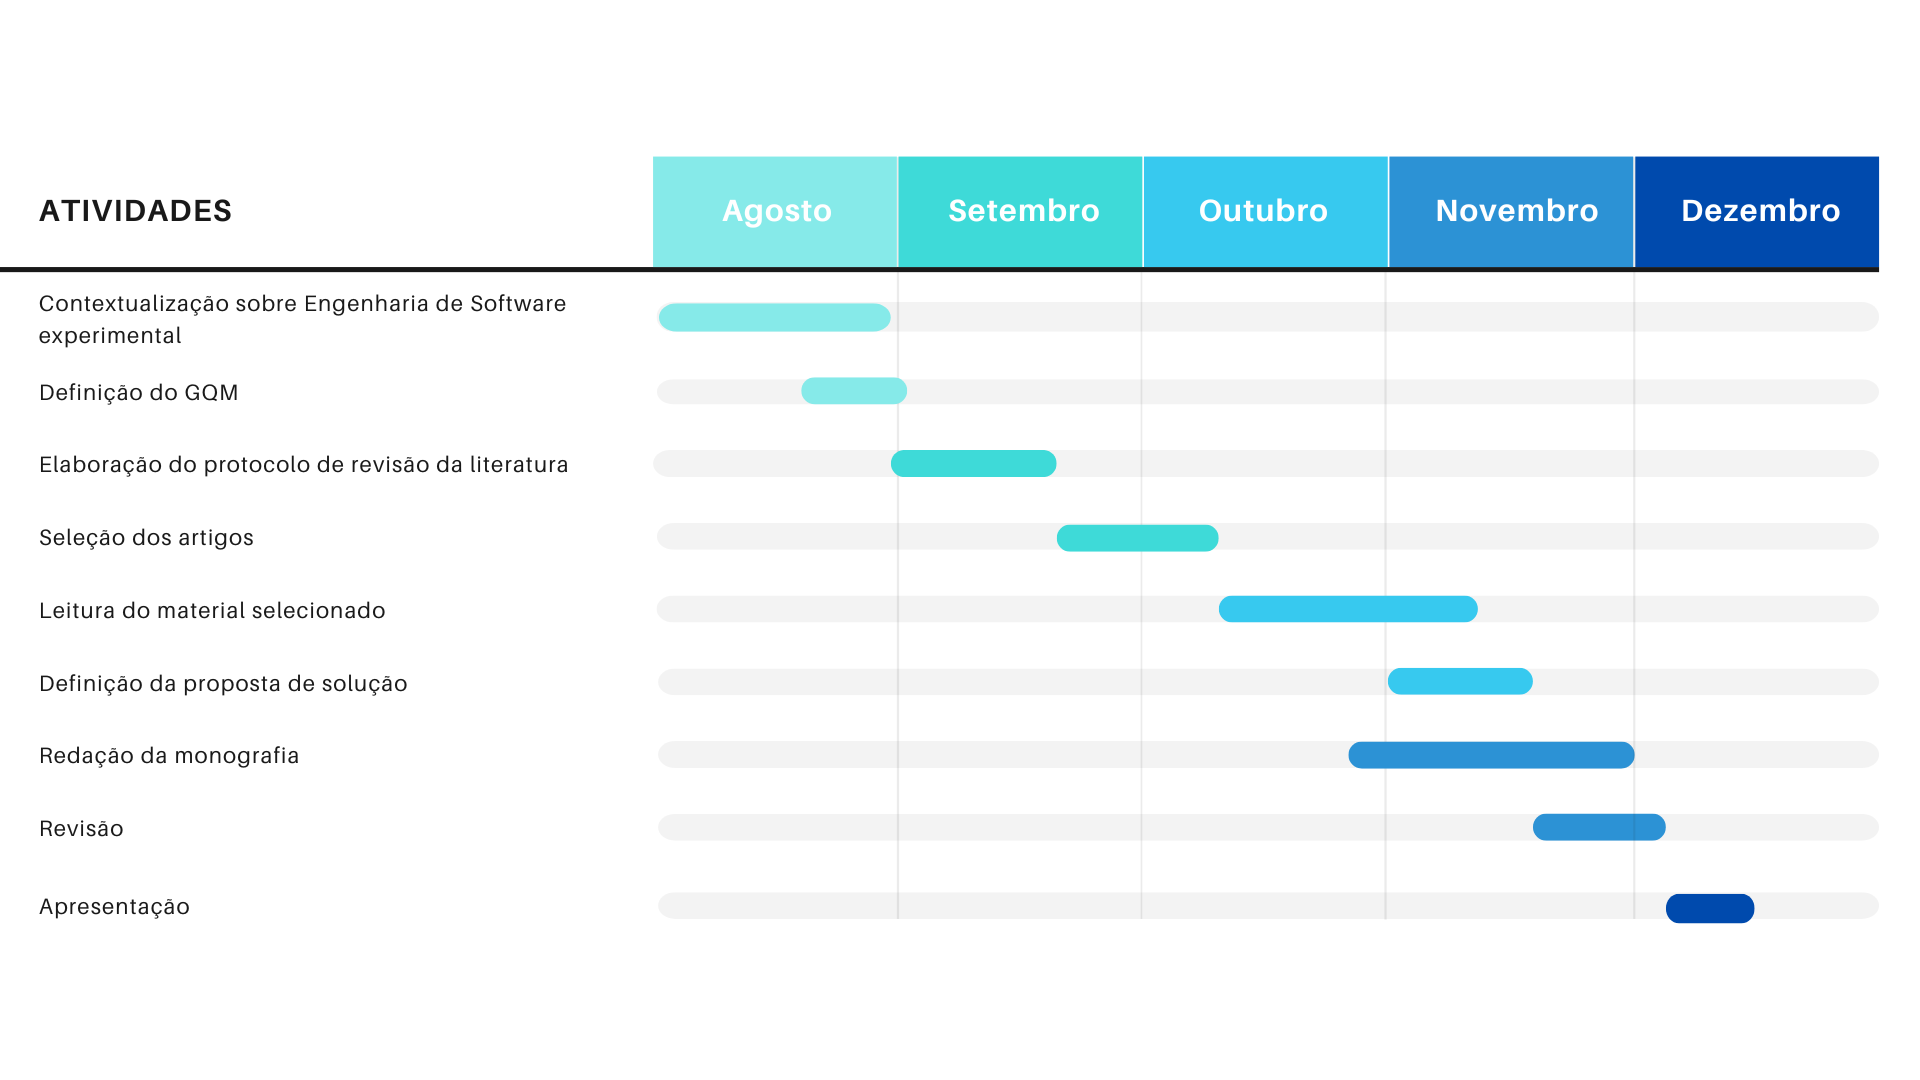
\includegraphics[width=1.1\textwidth]{figuras/CronogramaAtividades.png}

    \label{fig:cronograma}
	Fonte: Autor
\end{figure}